\documentclass[11pt,a4paper]{article}

% --- Packages de Base ---
\usepackage[utf8]{inputenc}
\usepackage[T1]{fontenc}
\usepackage{geometry}
\usepackage{graphicx}
\usepackage{xcolor}
\usepackage{tcolorbox}
\usepackage{hyperref}
% --- En-têtes et Listes ---
\usepackage{fancyhdr}
\usepackage{lastpage}
\usepackage{enumitem}
\usepackage{titlesec}
\usepackage{booktabs}
\usepackage{svg}
\usepackage{tabularx}
\usepackage{array}
\usepackage{subcaption}
% biblio
\usepackage[
backend=bibtex,
style=numeric,
sorting=nty
]{biblatex}

\addbibresource{biblio.bib}
\geometry{top=2.5cm, bottom=2.5cm, left=2.5cm, right=2.5cm}
% --- Définition de Couleurs ---
\definecolor{darkblue}{RGB}{92, 48, 110}
\definecolor{lightgray}{rgb}{0.95, 0.95, 0.95}
\definecolor{linkrose}{RGB}{175, 106, 140}
% --- Graphismes et Couleurs ---

\hypersetup{
    colorlinks=true,
    linkcolor=linkrose,
    citecolor=linkrose,
    filecolor=black,
    urlcolor=black,
    pdftitle={ErwannGallois},
    pdfpagemode=FullScreen,
}

\usepackage[toc]{glossaries}
% \makeglossaries
\makenoidxglossaries
\newacronym{rna}{RNA}{RiboNucleic Acid}
\newacronym{rasp}{RASP}{Ribonucleic Acids Statistical Potential}

% \renewcommand{\glstextformat}[1]{\color{black}  #1}
\renewcommand{\glstextformat}[1]{\color{blue}  #1}


\renewcommand{\glstextformat}[1]{\textcolor{linkrose}{#1}}



% --- Mise en page des titres ---
\titleformat{\section}{\large\bfseries\color{darkblue}}{\thesection}{1em}{}[\titlerule]
\titleformat{\subsection}{\normalsize\bfseries\color{darkblue}}{\thesubsection}{1em}{}
\titleformat{\subsubsection}{\normalsize\color{darkblue}}{\thesubsubsection}{1em}{}

% --- Configuration En-tête / Pied de page ---
\pagestyle{fancy}
\fancyhf{}
\setlength{\headheight}{14pt}
\renewcommand{\headrulewidth}{0.4pt}
\renewcommand{\footrulewidth}{0.4pt}
\lhead{\color{gray}Internship Report}
\rhead{\color{gray} GALLOIS Erwann}
\cfoot{\thepage / {\hypersetup{linkcolor=black}\pageref{LastPage}}}

\fancypagestyle{plain}{%
    \fancyhf{}
    \setlength{\headheight}{14pt}
    \renewcommand{\headrulewidth}{0.4pt}
    \renewcommand{\footrulewidth}{0pt}
    \lhead{\color{gray}Internship Report}
    \rhead{\color{gray} GALLOIS Erwann}
}

% --- Informations du Document ---
% \title{
%     \vspace{2cm}
%     \HRule \\[0.4cm]
%     \huge \bfseries \color{darkblue} Title of the Internship \\
%     \large M2 Internship Report \\
%     \HRule \\[1.5cm]
% }
% \author{\textbf{GALLOIS Erwann} \\[0.5cm]
% \small { \textbf{Internship tutors :} M. POSTIC Guillaume} \\
% \small { \textbf{Referent teacher :} Ms. BOURDACHE Nadjet}
% }
% \date{ }

\newcommand{\HRule}{\rule{\linewidth}{0.5mm}}

% ==========================================
% DEBUT DU DOCUMENT
% ==========================================
\begin{document}

\begin{titlepage}
   \begin{center}
        \vspace*{2cm} % Adjust spacings to ensure the title page is generally filled with text
        %% input logos
        % {\includegraphics[width=0.22\textwidth]{images/logo/univ-rouen.jpg} \quad \quad}{\includegraphics[width=0.2\textwidth]{images/logo/lmrs.png} \quad \quad}
        % {\includegraphics[width=0.11\textwidth]{images/logo/cnrs.png}}\\
        {
\includegraphics[width=0.3\textwidth]{img/LOGO-UNICAEN_V-2.1-N.png} \quad}
        \noindent\rule[0.25\baselineskip]{\textwidth}{1pt}
        
        \vspace{0.5 cm} 

        \Huge{\textbf{Internship Report}}\\ 

        \vspace{0.5cm}
        \LARGE{Prediction of RNA 3D structure using gradient-descending and knowledge-based scoring function}
          
        \vspace{2 cm}
        % \Large{\GroupName}
        \vspace{0.25cm}
        \large{\textbf{GALLOIS Erwann}}\\
        \large{Internship carried out from 02/03/2026  to  04/09/2026}\\
        % \vfill
        \vspace{4 cm}
         
        \leftline{ \small { \textbf{Internship tutors :} M. POSTIC Guillaume}}
        \leftline{ \small { \textbf{Referent teacher :} Ms. BOURDACHE Nadjet}}
        \vspace{1 cm}
        \leftline{\small { \textbf{\'Educational institution :} Université Caen-Normandie / M2 IA, Santé et Sciences des Données}}
        \leftline{\small { \textbf{Internship host company :} IBISC (AROBAS) - Bâtiment IBGBI, 23 Bd de France 91034 Evry}}
        
        \noindent\rule[0.25\baselineskip]{\textwidth}{1pt}\\
        
        {
\includegraphics[width=0.4\textwidth]{img/logo_ibiscsaclay_bleu_324ptx89pt.png}\quad}
        % {\includegraphics[width=0.23\textwidth]{images/logo/saclay.png}\quad}\\
      
    \end{center}
\setcounter{page}{0}
\end{titlepage}
\thispagestyle{empty}
\newpage

% ==========================================
% Abstract
% ==========================================
\begin{abstract}
\thispagestyle{plain}
\noindent
Write an abstract here. \\  \\
\textit{Key words}: financial models, machine learning...
\end{abstract}

\newpage
\setcounter{page}{0}
\thispagestyle{plain}
{\hypersetup{linkcolor=black}
\tableofcontents}
\newpage

\setcounter{page}{1}
% ==========================================
% Présentation Entreprise
% ==========================================
\section{Presentation of the company}

The IBISC (Informatic, Bio-Informatic, System Complex) laboratory was founded in 2006, is a multidisciplinary research unit affiliated with the University of Evry Paris-Saclay. IBISC have two sites, Pelvoux and IBGBI. Its core scientific mission centers on the developpement of formalisms, algorithm, and computational methods to identify, optimize and validate complex system. 

The laboratory's research identity have two axes : "STIC \& Smart Systems" dedicated to artificial systems sush as ambient robotics and communication networks, and "STIC \& Life Sciences" focused on biomedical assistance, precision medecine and computational biology. 

The laboratory is structured into four speicalized teams : 
\begin{itemize}
    \item COSMO : COmmunication, Specialisation and MOdeles
    \item IRA2 : Interaction, Réalité virtuelle \& Augmentée, Robotique Ambiante
    \item SIAM : Signal, Image, AutoMatique
    \item AROBAS : Algorithme, Recherche Operationnelle, Bio-informatique et Apprentissage Statistique
\end{itemize}

For the past 20 years, IBISC produced thousands of scholarly publications (journal articles, conference proceedings, theses, and HDR dissertations) on the HAL portal. The laboratory is particularly distinguished by its rigorous policy on research output. It regularly publishes reports on “high-impact publications.” In the laboratory’s terminology, this mark of excellence specifically refers to work accepted in : Journals ranked in the top 10\% of CiteScoreMetrics, international conferences classified as A or A* and innovation patents.

\begin{figure}[h!]
    \centering
    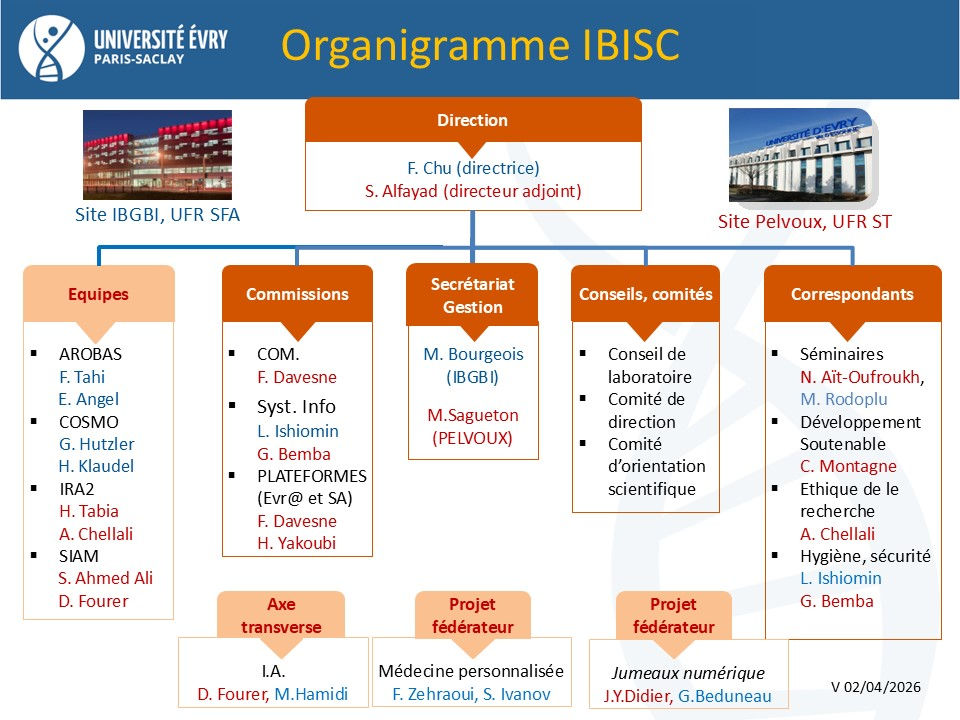
\includegraphics[width=0.95\textwidth]{img/Organigramme_IBISC-02042026.jpg}
    \caption{IBISC's organigram. Source : \cite{organigram}}
    \label{fig:organigram}
\end{figure}

% ==========================================
% Notion Préliminaires
% ==========================================
\newpage
\section{Preliminary notions}

The goal of this chapter is to give insights on preliminary notions that are important to comprehend my report. 

\subsection{Central Dogma}

Every cells of every living being, excluding virus and a few exceptions, has \acrfull{dna}. This molecule contains the genetic information. It holds all information for an organism. However the \acrshort{dna} alone cannot do anything, it needs to be express in proteins. This process is called the central dogma of molecular biology \cite{crick_central_1970}.
For that, the cell perform two steps: 
\begin{enumerate}
    \item Transcription : This steps copy a part of \acrshort{dna} and transcribes it into a intermediate molecule called \acrfull{rna}, or more precisely messenger RNA (mRNA). The transcription is performed inside the nucleus.
    \item Translation : The RNA obtained in the previous step are now used to make a protein. The translation is performed outside of the nucleus.
\end{enumerate}

\begin{figure}[h!]
    \centering
    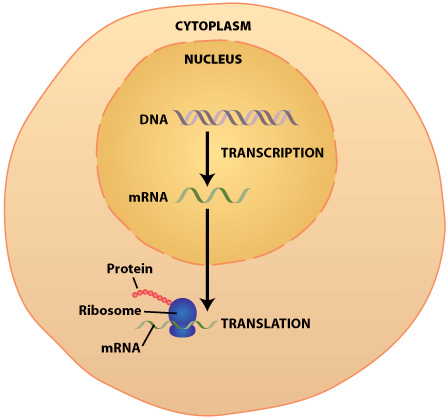
\includegraphics[width=0.4\textwidth]{img/protein-synthesis.jpg}
    \caption{A diagram illustrating the processes of \acrshort{dna} transcription into RNA and RNA translation into proteins. Source : \cite{duke_apep_dna}}
    \label{fig:protein-synthesis}
\end{figure}

Recently, researchers have discovered that RNA serves more than just an intermediate role. Indeed, many RNAs, known as non-coding RNAs, are never translated into proteins. Instead, they have a regulation role inside the cell.

\subsection{RNA molecule}

The RNA is single-stranded, unlike \acrshort{dna} which is double-stranded, and it's a polymer of nucleotids. The linear arrangement of these nucleotides defines it's primary structure (1D structure) or it's raw sequence. 
A nucleotide is composed by three components (Fig. \ref{fig:1d-structure}) : a nucleobase, a ribose sugar and a phosphate group. Unlike phosphate group and ribose sugar who is common for all nucleotides, the nucleobase determine the type of nucleotide. For the RNA, there are four types of nucleobases : Guanine (G), Adenine (A), Cytosine (C) and Uracil (U). 

\begin{figure}[h!]
    \centering
    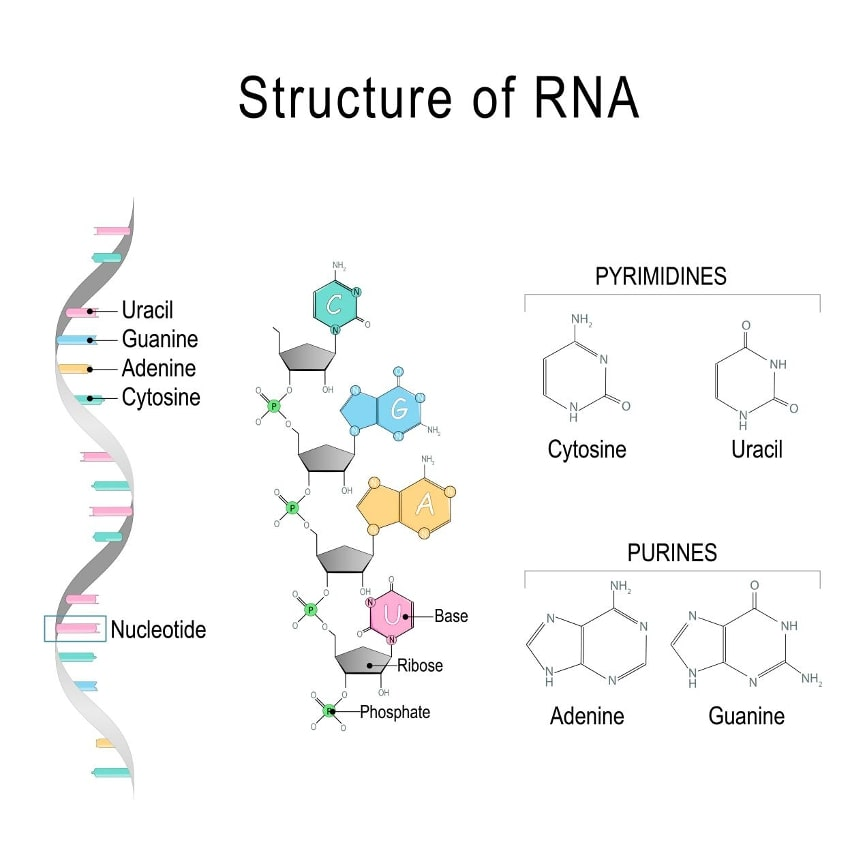
\includegraphics[width=0.6\textwidth]{img/1d-structure.jpg}
    \caption{A diagram illustrating the 1D-structure of RNA and nucleotid composition. Source : \cite{bocsci_rna_bases}}
    \label{fig:1d-structure}
\end{figure}

There is two form of nucleobase : pyrimidines for uracil and cytosine, purines for adenine and guanine. Purines have a second ring, so they have more atoms and are bigger than pyrimidines. These nucleobase can assemblate by stacking on top of each other trought van der Walls interactions. There is also structural constraint influences by ribose sugar chain, this chain is called the backbone \cite{Montemayor:tb5151}. And finally, the phosphate group, carry negative energy so to neutralize this charges, RNA needs heteroatoms like ions or ligand to regulate it's energy. So the conformation of RNA it's very dependant of the environnement condition, it's surronding solvant and ions has a strong influences on it's stability and it's folding \cite{draper_rna_2008}.  

\subsection{RNA secondary structure}
\begin{figure}[h!]
    \centering
    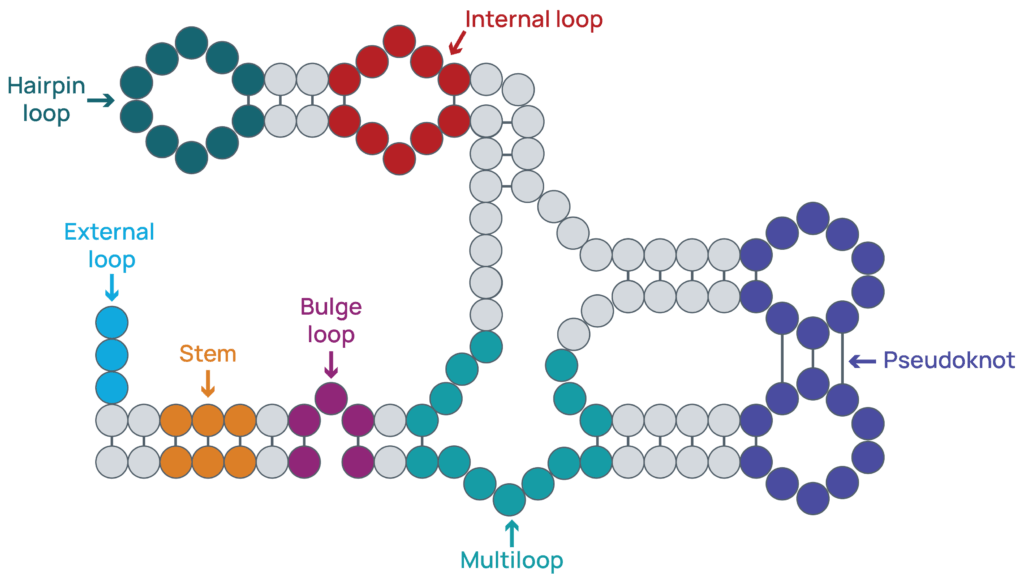
\includegraphics[width=0.4\textwidth]{img/2d-structure.png}
    \caption{A diagram illustrating different structural motifs . Source : \cite{eclipse-strucure}}
    \label{fig:2d-structure}
\end{figure}

The secondary or 2D structure is dictated by the primary structure. The 2D structure define the canonical interactions, such as Watson-Crick base pairing (A paring with U and G paring with C) and Wobble pair (G with U). The secondary structure alone can't define the folding of a RNA. Indeed, many pair can give multiple possible arrangement in 3D space (see Fig. \ref{fig:2d-structure}). 2D structure can also be driven by the RNA functions and interactions with proteins or other molecules. Like for 1D structure, the secondary structure influence completely the 3D structure, so knowing the RNA secondary structure for make a prediction can be effective and having a better accuracy. 

\subsection{RNA tertiary structure}

The transition from the secondary structure to the tertiary structure, or 3D structure, is determined by the geometric and topological properties of the motifs formed in the previous step. These motifs such as loops or bulges act as flexible hinges and anchor points.

Thanks to the flexibility of these nodes, the strand continues to fold. Long-range interactions then arise between 2D motifs that may be very far apart along the 1D structure but are geometrically close to one another in space. For example, a loop located at one end may interlock with the cavity of another region.

It is this dense network of interactions between the different motifs that forces the RNA to fold in a highly specific manner to adopt its final three-dimensional structure. In biology, a fundamental principle dictates that structure determines function. The tertiary structure allow the RNA molecule to interact with other element from the cell. 

So to know the folding and the function of a RNA we need to know the 1D structure (\ref{fig:1d-struc-3DIQ}). This will be used to determine the secondary structure (\ref{fig:2d-struc-3DIQ}), to finally predict the 3D structure (\ref{fig:3d-struc-3DIQ}). 

\begin{figure}[h!]
\begin{subfigure}{0.5\textwidth}
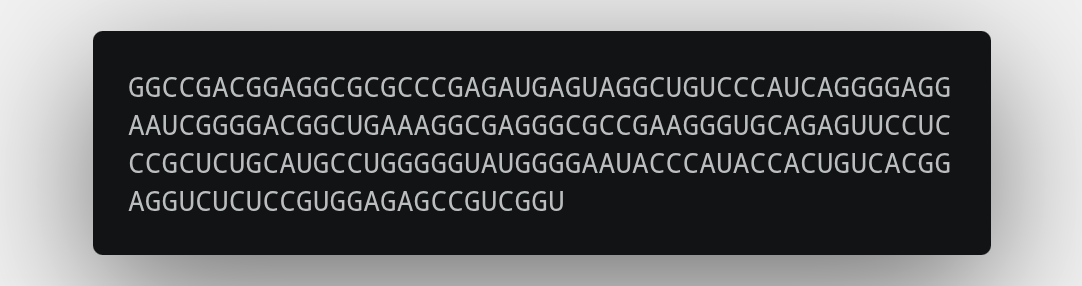
\includegraphics[width=0.9\linewidth]{img/3DIQ-1D.png} 
\caption{1D structure}
\label{fig:1d-struc-3DIQ}
\end{subfigure}
\begin{subfigure}{0.5\textwidth}
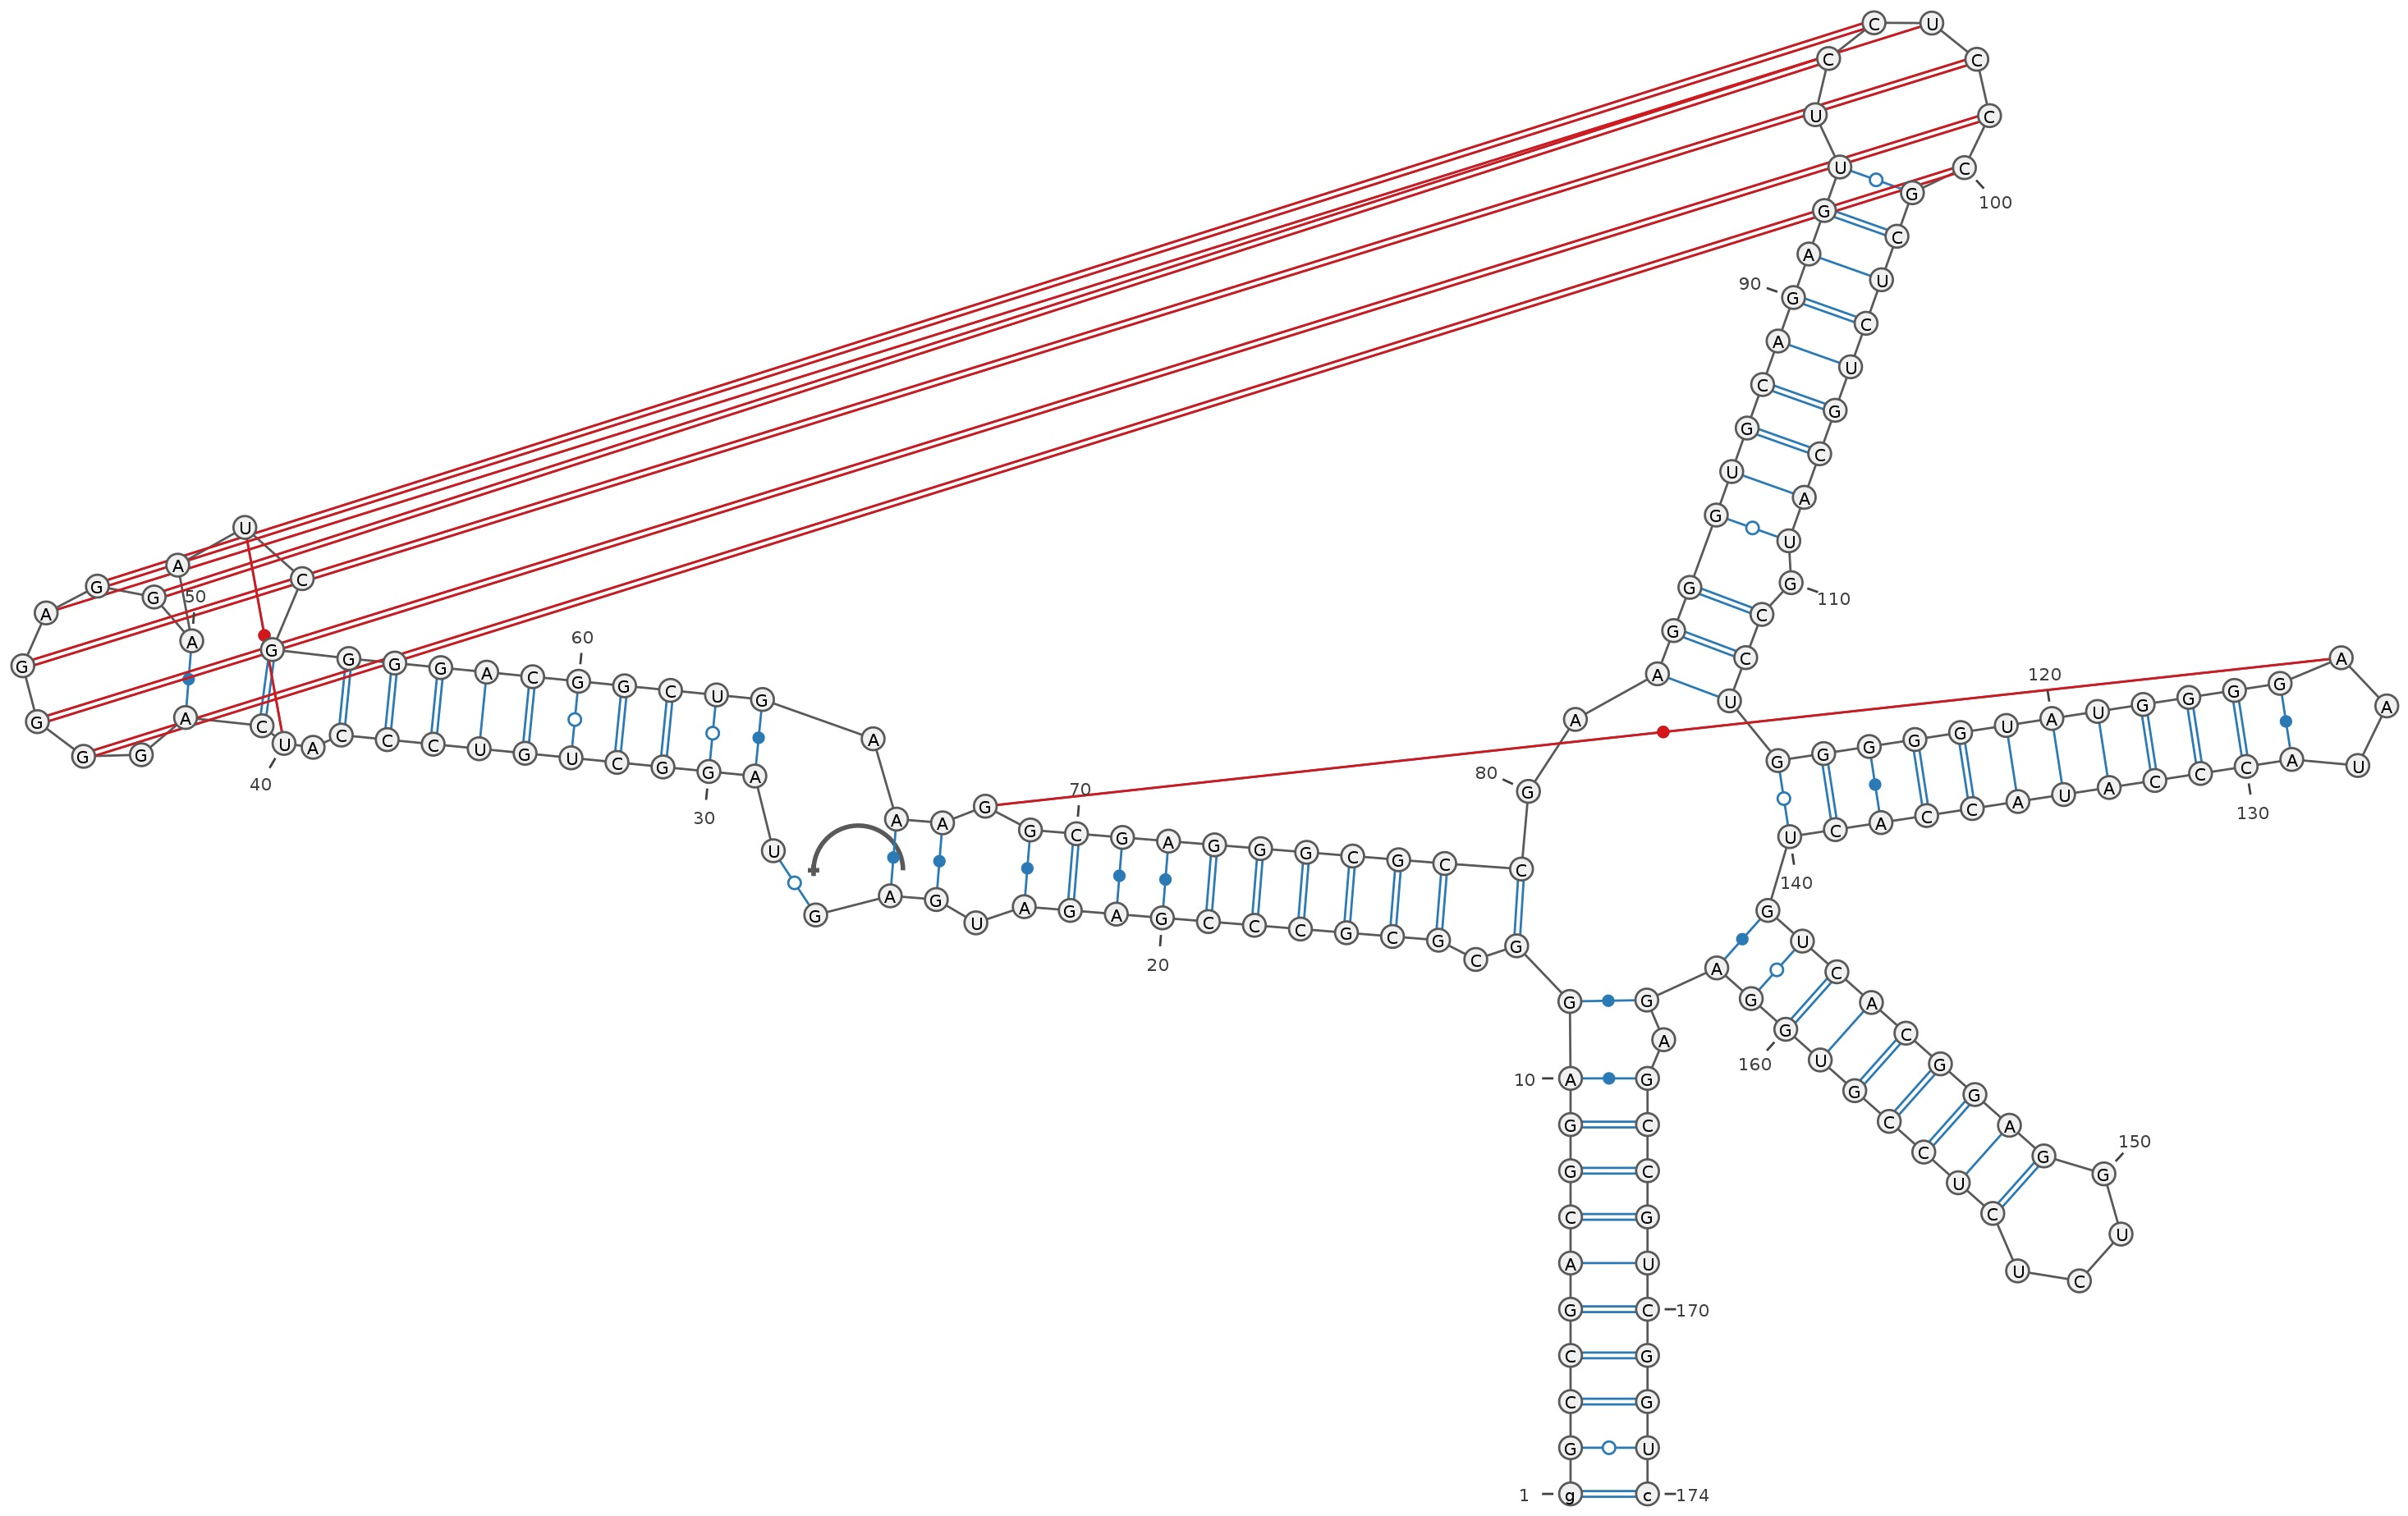
\includegraphics[width=0.9\linewidth]{img/3DIQ-2D.jpg}
\caption{2D structure}
\label{fig:2d-struc-3DIQ}
\end{subfigure}
\begin{subfigure}{0.5\textwidth}
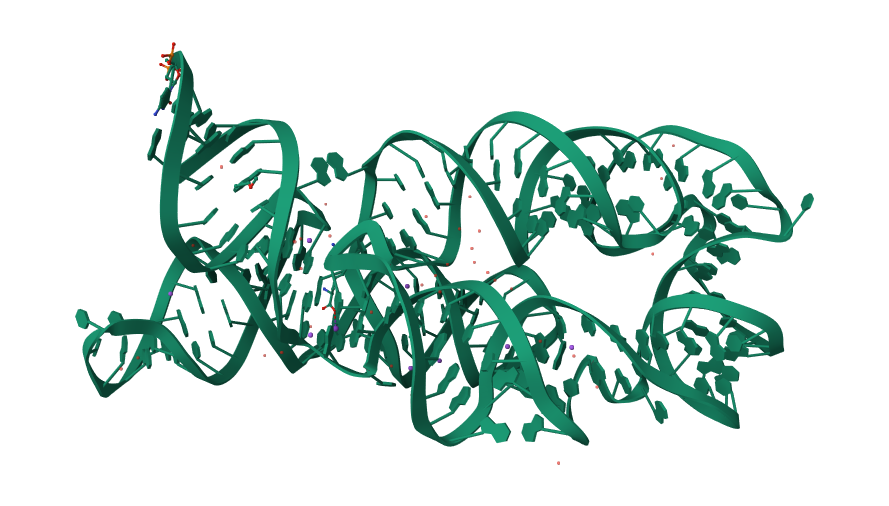
\includegraphics[width=0.9\linewidth]{img/3DIQ-3D.png}
\caption{3D structure (Cartoon representation)}
\label{fig:3d-struc-3DIQ}
\end{subfigure}

\caption{The three different level of representation for the same RNA (PDB ID : 3DIQ)}
\label{fig:image2}
\end{figure}

% ==========================================
% Introduction
% ==========================================
\newpage 
\section{Introduction}

\acrfull{rna} have a central and versatile role in cells. In addition  of messenger RNA, who are coding RNA, there are also non-coding RNA, such as transfer RNAs, ribosomal RNAs, micro RNAs. These non-coding RNA  regulates gene expression at transcriptional, post-transcriptional and translation level. Also, they catalyzes biochemical reactions, guides chemical modification of other RNAs \cite{cech2014noncoding, breaker2012riboswitches}. 

Crucially, the biological function of these molecule are not only dictated by it's sequence but especially from the tertiary structure into which they fold. As with proteins, structure determines function. For example, the ligand-binding pocket of a riboswitch or the recognition surfaces that mediate RNA-protein and RNA-small-molecule interactions all depend on precise tertiary structure. This structure-function association have a growing interest in RNA as a therapeutic target. 

For example, a riboswitch is cis-acting RNA elements that fold into a specific 3D pocket capable of binding a small molecule to trigger a conformational rearrangement of the RNA that switches downstream gene expression on or off, without any protein required \cite{warner2018principles}. Moreover, the FMN riboswitch can detect the intracellular levels of flavin monocleotide and when bound can regulate the \textit{ribB} gene. This gene is required for the vitamin B2 biosynthesis in bacterium. This regulation permits to the bacterium to shut down this costly pathway once enough vitamin B2 is availabled. 

Due to this regulator switch depends entirely on the riboswitch folding correctly into it's 3D structure, it, theoretically, can be design to be a drug and force the premature repression of the pathway. The repression can lead to a depletion of vitamin B2. Then this depletion will lead to downstream of FAD. These two molecules are essential for a bacterial growth. So without these two, this will lead to arrest bacterial proliferation and produce measurable antibacterial activity in vivo \cite{howe2015ribocil}.

Despite this importance, experimental determination of RNA 3D structures by X-ray crystallography, nuclear magnetic resonance spectroscopy, and cryo-electron microscopy remains laborious. Because RNAs are very flexable, also because there are highly charged and have flexible backbone \cite{wang2023trrosettarna}. The consequence is only around 6,000 RNA structures are deposited in the \acrlong{pdb}, far fewer than the roughly 190,000 deposited protein structures \cite{wang2023trrosettarna}. This structural gap has made computational prediction of RNA tertiary structure from sequence a pressing goal.

At first, computational RNA 3D structure prediction relied on two broad families of methods. Template-based approaches build models by reusing homologous fragments or full structures already present in the \acrlong{pdb}. Unfortunately, they fail for novel folds lacking known homologs. However, \textit{de novo} methods attempt to fold RNA from first principles: fragment-assembly approaches. For example, Rosetta's FARFAR2 assemble short structural fragments and refine them against an all-atom energy function \cite{watkins2020farfar2}. Besides there are also coarse-grained physics- and knowledge-based simulation methods, such as SimRNA sample conformational space, using Monte Carlo methods guided by a statistical potential \cite{boniecki2016simrna}. These approaches have been evaluated since 2011 through the community-wide, blind RNA-Puzzles experiment \cite{cruz2012rnapuzzles}. Their main limitations are the high computational cost of adequately sampling conformational space, a limitation of nucleotide number by a few hundred, and persistent inaccuracy in reproducing non-canonical base pairs and tertiary contacts.

The conceptual foundation for the deep-learning paradigm in structure prediction was laid by AlphaFold1, DeepMind's entry at CASP13 (2018). It have outperformed competing groups largely on the strength of a single algorithmic idea \cite{senior2020alphafold1}. Instead than assembling and screening large libraries of candidate fragments as prior methods did, AlphaFold1 trained a deep residual convolutional neural network to predict, from multiple sequence alignment-derived features, a probability distribution over the distance between every pair of residues and over the protein's backbone torsion angles. These predicted distributions were then combined into a single smooth, differentiable potential describing the whole protein chain. Then the 3D structure was obtained by directly minimizing this potential through gradient descent by using the same backpropagation machinery used to train the network. This meant that folding was no longer treated as a discrete search over sampled conformations, but as a continuous optimization problem solvable by following the gradient of a learned energy landscape toward its minimum, a strategy that proved both more accurate and computationally cheaper than actual methods at this time.
The 2021 successor, AlphaFold2 have achieved near-experimental accuracy in protein structure prediction \cite{jumper2021alphafold}. Thanks to AlphaFold1 and AlphaFold2 by proving that deep learning can be efficient for protein prediction, researchers decide too apply this technique into RNA. 

A first generation of RNA methods inspired by AlphaFold1, a neural network predicts geometric restraints from multiple sequence alignments,have emerged after the realease of it. For example DeepFoldRNA \cite{pearce2022deepfoldrna} folds RNA by applying the L-BFGS gradient descent algorithm directly to a potential built from its predicted geometric restraints, or trRosettaRNA \cite{wang2023trrosettarna} follows a closely related restraint-then-refine strategy. In the same way, DRfold \cite{li2023drfold} pushes this idea further by integrating end-to-end learning of local reference frames with deep geometric potentials within a single differentiable pipeline. 

AlphaFold2 inspired also other model by predicting atomic coordinates directly from sequence. Notably, RhoFold+ \cite{shen2024rhofold} combines an RNA language model pre-trained on over 23 million non-coding RNA sequences with a folding module. But also, NuFold \cite{kagaya2025nufold} who adapts the AlphaFold2 architecture with a flexible nucleobase-center representation, or RoseTTAFoldNA \cite{baek2024rosettafoldna} who extends the three-track RoseTTAFold architecture to nucleic acids and protein–nucleic acid complexes, and, most recently, AlphaFold3 \cite{abramson2024alphafold3} employs a diffusion-based architecture capable of jointly predicting proteins, nucleic acids, and small molecules.

Despite these advances, deep learning has not yet delivered for RNA the same progress than it produced for proteins. At CASP15, the first CASP round to formally assess RNA structure prediction, the top-ranked groups relied on knowledge-based energy potentials and manual conformational sampling rather than deep learning, and predictions from deep-learning approaches were found to be significantly less accurate than these expert, physics-based methods \cite{das2023casp15}. This pattern persisted at CASP16, where the assessors reported no notable increase in nucleic acid modeling accuracy from deep learning \cite{kretsch2025casp16}. Systematic benchmarking corroborates these findings: while machine-learning methods generally outperform fragment-assembly methods, both categories perform poorly on RNAs lacking detectable homologs and on non-canonical base-pairing interactions, which remain a shared point across all current methods \cite{bahai2024benchmarking}. The principal obstacles underlying these limitations are the scarcity of experimental RNA structures available for training relative to proteins, the frequent shallowness or absence of multiple sequence alignments for many RNA families, and the difficulty of capturing long-range tertiary motifs and conformational flexibility.

It is within this rapidly evolving but still maturing context, one in which deep learning has substantially accelerated and improved automated RNA structure prediction without yet matching the accuracy achieved for proteins, that the present work is situated.

Instead of training a new neural network, because its still fundamentally constrained by the number of experimental RNA structures, this internship explores an alternative route. Indeed, we will directly optimizing a physically plausible RNA conformation against a knowledge-based statistical potential through gradient descent, like for the AlphaFold1's idea. The central obstacle to this approach is that statistical potentials are tabulated, discontinuous functions and are therefore not directly compatible with gradient-based methods. We overcome this problem by interpolating the potential using Catmull-Rom splines. We also used a coarse-grained bead-spring representation of the RNA, with bonded and steric energy terms, to accelerate calculation. The resulting objective function is minimized with a hybrid optimization strategy that pairs local exploration via the Adam algorithm with a basin-hopping-inspired global search, so as to escape the numerous local minima introduced by the interpolated potential.

% ==========================================
% Data and Dataset
% ==========================================
\newpage
\section{Data and Dataset}
\subsection{PDB database}

The \acrfull{pdb} \cite{berman2000pdb,rcsb2025pdb} is the principal worldwide archive for three-dimensional structures of biological macromolecule such as proteins and nucleic acids. This database centralize all structure determined by experimental methods such as X-ray crystallography, nuclear magnetic resonance spectroscopy and cryo-electron microscopy. It can be accessed through its website and an API. Each structure has an identifier composed of four letters or numbers (e.g. 1J8G) and they can be download in two format : PDB file and \acrfull{cif} files. A format change happen in 2014, with the advent of cryo-electron microscopy, researchers had the tools to see larger molecules like RNA polymerase. These types of molecules have a lot of atoms but PDB file are restricted to only 99 999 atoms, with mmCIF files, there is no limit on the molecule's scale. As a result, every new molecule added to the database is now in this format. These two format will be describe in the next section. 

\subsection{PDB file structure}
The PDB file is a file to represent each atom from a molecule, especially for protein and RNA. Each line have a keywords to explicite the line content. The file can be split in 3 parts. 

The first one contains header and metadata. This part have all information about the molecule and the experimentation.
\begin{table}[h!]
\centering
\small
\setlength{\tabcolsep}{4pt}
\begin{tabularx}{\textwidth}{|>{\raggedright\arraybackslash}p{2.5cm}|>{\centering\arraybackslash}X|}
\hline
Keywords & Description                            \\ \hline \hline
HEADER   & Molecule Type, PDB Id, deposition date \\
TITLE    & Title of the experiment                \\
COMPND   & Description of the molecule compenent  \\ 
SOURCE   & Biological origin or Synthetic \\
KEYWDS & Descriptive keywords for the structure \\
EXPDTA & Experimental Methods \\
AUTHOR & Author of the deposit \\
REVDAT & Revision history \\
JRNL & Publication reference \\
REMARK & Comments numbered from most important to least important \\
\hline
\end{tabularx}%
\caption{All keywords founded in a first part of a PDB files}
\label{tab:pdb-first-part}
\end{table}

The table \ref{tab:pdb-first-part} present all keywords and his signification. REMARK contains useful information such as the resolution of the molecule. The resolution is the difference between the atoms found experimentally and the actual atoms. More the resolution is low, more the experimental molecules can be accurate. 

The second part are about the sequence and the crystallography parameters. These keywords are all in the table \ref{tab:pdb-second-part} 

\begin{table}[h!]
\centering
\small
\setlength{\tabcolsep}{4pt}
\begin{tabularx}{\textwidth}{|>{\raggedright\arraybackslash}p{2.5cm}|>{\centering\arraybackslash}X|}
\hline
Keywords & Description                            \\ \hline \hline
SEQRES   & Primary Sequence by chain \\
CRYST1    & Crystal lattice parameters                \\
SCAL1/2/3   & Orthogonal coordinate conversion matrices  \\ 
\hline
\end{tabularx}%
\caption{All keywords founded in a second part of a PDB files}
\label{tab:pdb-second-part}
\end{table}

A chain in an alternative conformation for the same molecule, sometimes by adding some ligand or other molecules to induce the change of conformation. SEQRES can be used to find the acid nucleics sequence that can be retrieved and put inside a algorithm to predict the three-dimensional structure. 

The last part is the goal of this file, the coordinates of every atoms from the molecule. This section is formatted in fixed columns. It's not just generic space between columns, the position is important. The information for every line is resume in the table \ref{tab:pdb-third-part}. 
\begin{figure}[h!]
    \centering
    
\includegraphics[width=\textwidth]{img/example-pdb.png}    
    \caption{Line 808 from the pdb file from the pdb id 1J8G \cite{deng_x-ray_2001}}
    \label{fig:ex-pdb}
\end{figure}


\begin{table}[h!]
    \centering
    \small
    \setlength{\tabcolsep}{4pt}
    \begin{tabularx}{\textwidth}{|>{\raggedright\arraybackslash}p{1.5cm}|>{\raggedright\arraybackslash}p{3.0cm}|>{\raggedright\arraybackslash}p{2.5cm}|>{\raggedright\arraybackslash}X|}
        \hline
        Columns & Fields & Value (from Fig. \ref{fig:ex-pdb}) & Description\\ \hline \hline
        1-6   & Record Name & \verb|ATOM| & Two types: \texttt{ATOM} for standard residues and \texttt{HETATM} for heteroatoms \\
        7-11  & Serial Number & \verb|1| & Sequential atom number \\
        13-16 & Atom Name & \verb|O5'| & Atom name per IUPAC nomenclature \\
        17    & AltLoc & blank & Alternate location indicator, used when an atom has more than one modeled conformation (A/B) \\
        18-20 & Residue Name & \verb|U| & Residue type (e.g. uracil for RNA) \\
        22    & Chain ID & \verb|A| & Chain identifier \\
        23-26 & Residue Sequence Number & \verb|1| & Residue position within the chain \\
        31-38 & x & \verb|12.967| & Cartesian X coordinate (\AA) \\
        39-46 & y & \verb|20.885| & Cartesian Y coordinate (\AA) \\
        47-54 & z & \texttt{19.962} & Cartesian Z coordinate (\AA) \\
        55-60 & Occupancy & \texttt{1.00} & Fraction of the unit cell in which this atom occupies this position (1.00 = always present) \\
        61-66 & Temperature Factor & \texttt{5.19} & Thermal displacement / positional uncertainty (B-factor); lower = sharper, more ordered atom \\
        77-78 & Element & \texttt{O} & Chemical element symbol \\
        \hline
    \end{tabularx}
    \caption{All keywords found in the coordinate section of a PDB file}
    \label{tab:pdb-third-part}
\end{table}

\subsection{Difference between PDB file and mmCIF file}

PDB files and mmCIF files have the same goal: describe the structural content. They have the same type of information, coordinates, experimental metadata. For the same PDB id, these two files must describe exactly the same molecule. The difference between them is not about the information but about the structure file.

A PDB file uses fixed-width columns, so a parser needs to know exactly the specification. On the contrary, mmCIF is a key-value format, where each value is explicitly named. This format is more general and can be used by more tools and more easily. Because each value is a free token instead of a fixed-width column, mmCIF has no limit on chain ID length or residue number, which is why it can scale to every molecule, even massive assemblies like ribosomes or cryo-EM structures that a PDB file cannot represent. On the other hand, a mmCIF file is less user-friendly when you want to read information without a parser. These differences between these file types explain why both extensions are usually available inside the PDB database, except for very large structures where only mmCIF can be provided.


% ==========================================
% Materials and Methods
% ==========================================
\newpage
\section{Materials and Methods}
\subsection{Knowledge based potential}

A knowledge based potential or statistical potential is a empirical scoring function. Indeed, she comes from a statistical analyses from 3D structures coming from the PDB. Unlike the physical potential, who based on fundamental laws of molecular mecanisms, a knowledge based score function is based on Bolzmann inversion principle. It posits that the frequency with which a given structural feature occurs in nature reflects its free-energy state, a theoretical approach initially formalised for macromolecules in the work of Miyazawa and Jernigan \cite{Miyazawa1985EstimationOE} and Sippl \cite{sippl_calculation_1990}.

In case of RNA, the statistical potential compares the special conformation frequency, like interatomic distances or  torsion angles, and a reference random distribution. If a interaction is observed significantly more often that randomly, then we attribute a favorable negative energy score, and if the interaction is rare, she have a penality. 

In this internship, we compared four different statistical potential. There are all distance-based potentials, meaning we cannot used it for torsion angles.  

\begin{itemize}
    \item \acrfull{rasp} \cite{capriotti_all-atom_2011}: It's using a simplify full-atom (23 atoms type) representation and a standard statistical reference.
    \item \acrfull{dfire} \cite{zhang_all-atom_2020} : It's using a all full-atom (85 atoms type) representation and used a another representation based on finite ideal gas. This representation eliminates the spacial biais. 
    \item \acrfull{rsrnasp} \cite{tan_rsrnasp_2022} : Unlike DFIRE-RNA and RASP, it's based on the fact that the RNA folding is hierarchical. Indeed the interaction between neighbour nucleotids do not obey the same geometric constraint as interactions between nucleotides that are further apart in the sequence. So this potential, use the all full-atom representation. It's calculates distinct energy potentials based on the sequential distance between two atoms. 
    \item \acrfull{cgrnasp} \cite{tan_cgrnasp_2023} : It's using the same approach as rsRNASP but changes the representation using only few atoms, less than 10 atoms, to represents all the nucleotides. 
\end{itemize}

\subsection{Representation}

To represents the RNA, we used a bead-springs representation or coarsed-gained representation, that means to represent the nucleotids we used only one atom and every atoms are connected by a spring.  This representation is more faster than a full-atom representation but less precise. But with this representation, we need to decide which atom, from the nucleotide, we will used. To resolve this problem, we selectionned three atom : 
\begin{itemize}
    \item C3' : We selected this atom because it's fixation point of the phosphate group. It's the topology equivalent of the alpha carbon for the protein. This atom is centered on the backbone sugar-phosphate. The C3' sequence provides an extremely smooth geometric representation of the RNA chain. It's privilaged choice used by model like NAST \cite{jonikas_coarse-grained_2009} who using also the single-atom representation.
    \item C4' : With this atom, the representation retains a very precise spatial memory of the local conformation of the cycle. Moreover, the inter-C4' distance mathematically better reflect the local curvature constraints of the phosphodiester chain than C3' does. 
    \item C1' : The C1' represent the glycosidique bond. This bond connects the ribose backbone to the nucleobase. Also, distance between two opposed C1' is symetrical, invariant and predicatable in a Watson-Crick pairing. Unlike C3' and C4', who are atom references, with the C1' we can see if the optimization algorithm can maximize the accuracy of secondary and tertiary matches by minimizing the energy. 
\end{itemize}


\subsection{Objective function}

The objective function will be used in a gradient descending optimisation. So it's need to be continuous and derivable. But, as we see before a knowledge based potential it's not derivable and continuous. Indeed it's only a matrix with energy depending on the distance and two atoms. So to bypass ths problem, we used a Catmull-Rom interpolation. It's a mathematical geometric modeling technique used to create a smooth cubic curve, that passes trought the point from the matrix of the potential. The fundamental property of this model lies in the automatic calculation of the tangent at each points $P_i$, which is defined to be strictly collinear with the vector connecting the adjacent points $P_{i-1}$ and $P_{i+1}$. Thanks to this property, the curve we obtained is continuous and derivable, and can be used in a gradient descending.

To represents the RNA, we used a bead-springs representation or coarsed-gained representation, that means to represent the nucleotids we used only one atom and every atoms are connected by a spring.  This representation is more faster than a full-atom representation but less precise. But with this representation, we need to decide which atom, from the nucleotide, we will used. To resolve this problem, we selectionned three atom : 



\begin{equation}
    w_1 * \text{Potential Statistical} +  w_2 * (k * \sum_{1}^{n-1}(l_0 - r)^2) + w_2  * WCA
    \label{eq:bead-springs}
\end{equation}

\begin{equation}
    WCA = 
    \begin{cases} 
    \epsilon \left[ \left(\frac{r_{min}}{r}\right)^{12} - 2\left(\frac{r_{min}}{r}\right)^6 + 1 \right] & \text{si } r < r_{min} \\
    0 & \text{si } r \ge r_{min}
    \end{cases}
    \label{eq:wca}
\end{equation}

So the objective function (see Equation \ref{eq:bead-springs}) have three terms. The first one is the statistical potential using the interpolation. 

The second one is the Fraenkel potential, it's used to regulate the springs compression and it's a constant so it's doesn't influence the continuous and derivability of the function. Indeed this term, have four constant, the $n$ is the number of nucleotids. Then, the $l_0$ is equilibrium length, it's where the springs have no force, no energy. Next, the $r$ is the instentaneous distance between two beads. Finally, the $k$, it's the stiffness constant, defines the diffuculty to compress or strecth the springs. 

The last one, it's the \acrfull{wca} potential (see Equation \ref{eq:wca}), this potential is a trunked version of the Lennard-Jones potential \cite{lennard-jones_cohesion_1931}. We include this term to avoid steric clash. Indeed this terms is only active when two beads are too close. This function is important because we doesn't influence the knowledge-based potential. To achieve this goal, there are three constant, the $r$, it's the euclidienne distance between two atoms. Then, the $r_{min}$, it's the minimal distance where the potential energy is minimal. And the $\epsilon$ represent the depth of the energy well of the original potential. The term $+1$ ensures that the energy vanishes continuously at $r =r_{min}$. 

Thanks to the interpolation and the others terms, the objective function can ensure that no physical laws are being violated. So the results can be used to other application. Since a present you the objectivefunction, i will now present you my algorithm. 

\subsection{Optimization algorithm}

The goal of the optimization algorithm is to find minimizing the objective function, because a find the most thermodynamically stable structure, the energy must be minimal. So to navigate through the complex energy landscape and find this minimal energy, we combined a local exploration via gradient descent and a global exploration inspired by the bassin-hopping algorithm. 

\subsubsection{Local exploration}

For the local exploration (see Fig.\ref{fig:local-optim}) we used the Adam optimization algorithm \cite{kingma2017adammethodstochasticoptimization}, unlike the AlphaFold 1, who used the \acrfull{lbfgs} optimization algorithm \cite{liu_limited_1989}. In fact, in our case, we start from a linear structure and we try to folding it. But the L-BFGS converge fast to the first local minimum, however a knowledge-based potential have a lot of minimum local due to the interpolation. Also Adam doesn't make assumptions about curvature, on the contrary the L-BFGS who constructs its approximation of the Hessian based on the history of gradient differences. Therefore, we used the Adam optimization to resolve our problem. 

At each iteration, the algorithm calculates the total energy of the system and performs a backpropagation to obtain the energy gradients with respect to the spatial coordinates of the atoms. These gradients are the physical forces acting on the molecule. We have also add a numerical stability to avoid a explosion of the molecule when we have a steric clash during the foldin, by adding a gradient clapping mechanism, capping the gradient norm at a maximum value. 

To not have a endless loop, we have a two security. The first one is a maximum of cycle, and the second one, is a \textit{local patience}. If the energy decrease between steps falls below a minimum tolerance threshold, then we add $+1$ to a counter until the algorithm reach the \textit{local patience}, and stop early the local exploration, at the end we have a phase score. 

The last problem of this local optimization is the data transfers between the \acrfull{cpu} and the \acrfull{gpu} who slow down the optimization. To mitigate this, the algorithm groups execution of local optimization steps into blocks. During a execution of a block, every calculation are performed on GPU. The retrieval of energy values to the CPU only occurs at the end of the block. This technique helps to avoid a bottlenecks between the GPU and CPU. 

\begin{figure}[h!]
    \centering
    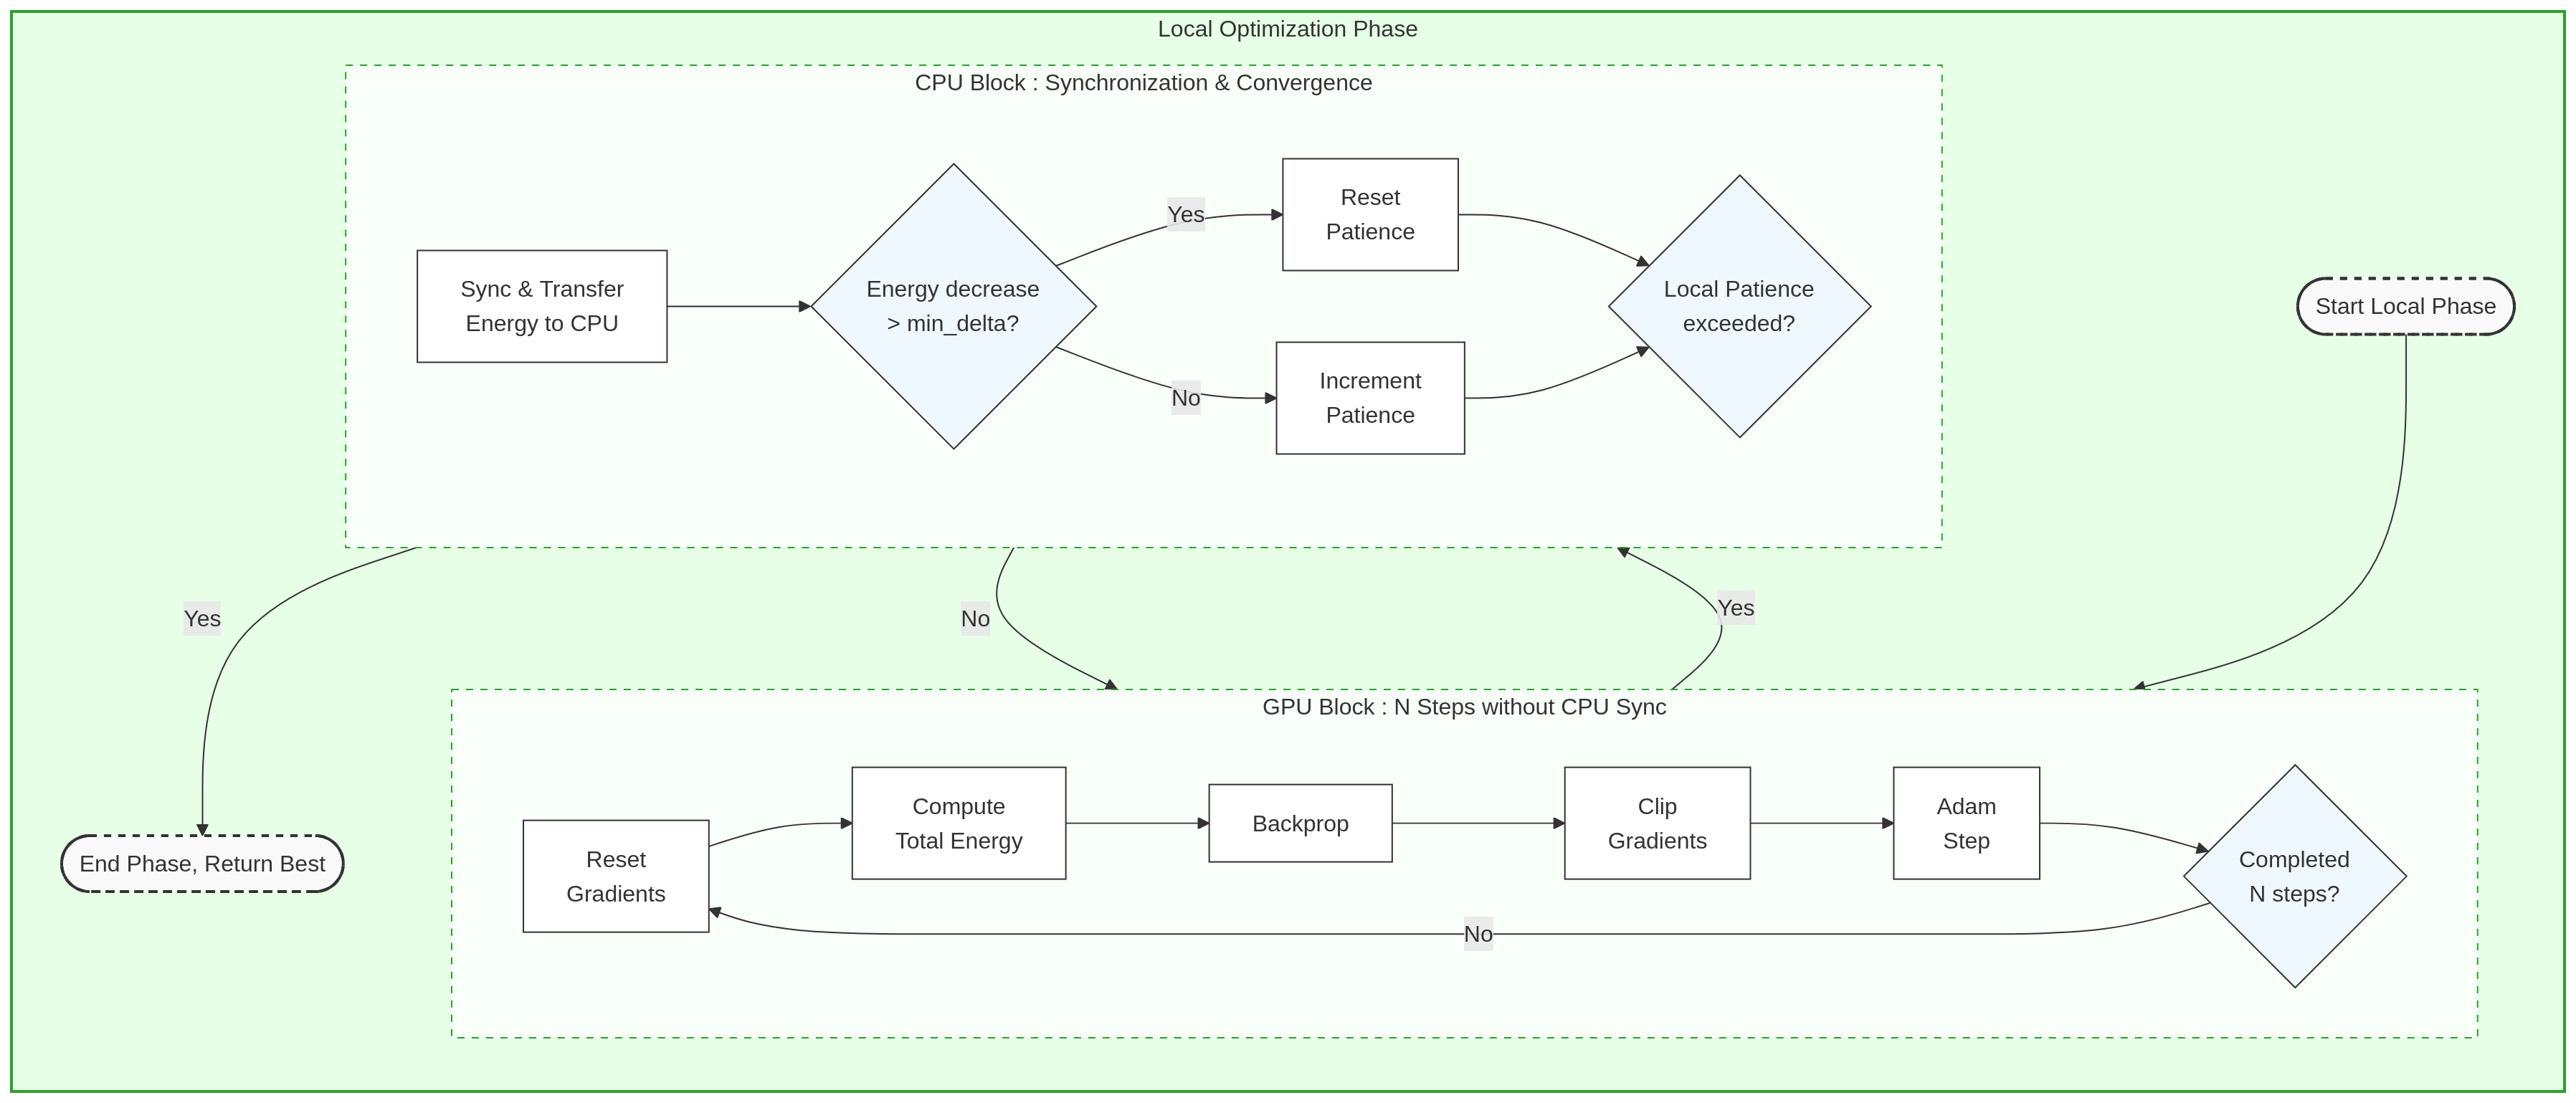
\includegraphics[width=\textwidth]{diagrams/local_optim.png}
    \caption{Local optimization phase (Adam gradient descent).}
    \label{fig:local-optim}
\end{figure}

\subsubsection{Global exploration}

As mentioned above, the statistical potential interpolation have a lot of local minima, and a gradient descending alone have tendency to be trapped in a local minima. To overcome this problem, we added a global optimization loop (see Fig. \ref{fig:global-optim}). 

When the local exploration has converged, the algorithm compared the phase score with the best historical score. It stores the best conformation, then applies a random geometric pertubation to the 3D coordinates. This noise ejects the structure from it's current local minimum. After that the noisy structure is send to a new local optimization phase. To not lose maybe a good structure, the amplitude of the pertubation decreases over the cycles according to a cooling factor. 

The global exploration terminates based on two criteria : either the noise amplitude reach a minimum threshold or the algorithm is no longer able to find a conformation with a global energy lower than the established record after several successive pertubation cycles, the \textit{global patience}.  

\begin{figure}[h!]
    \centering
    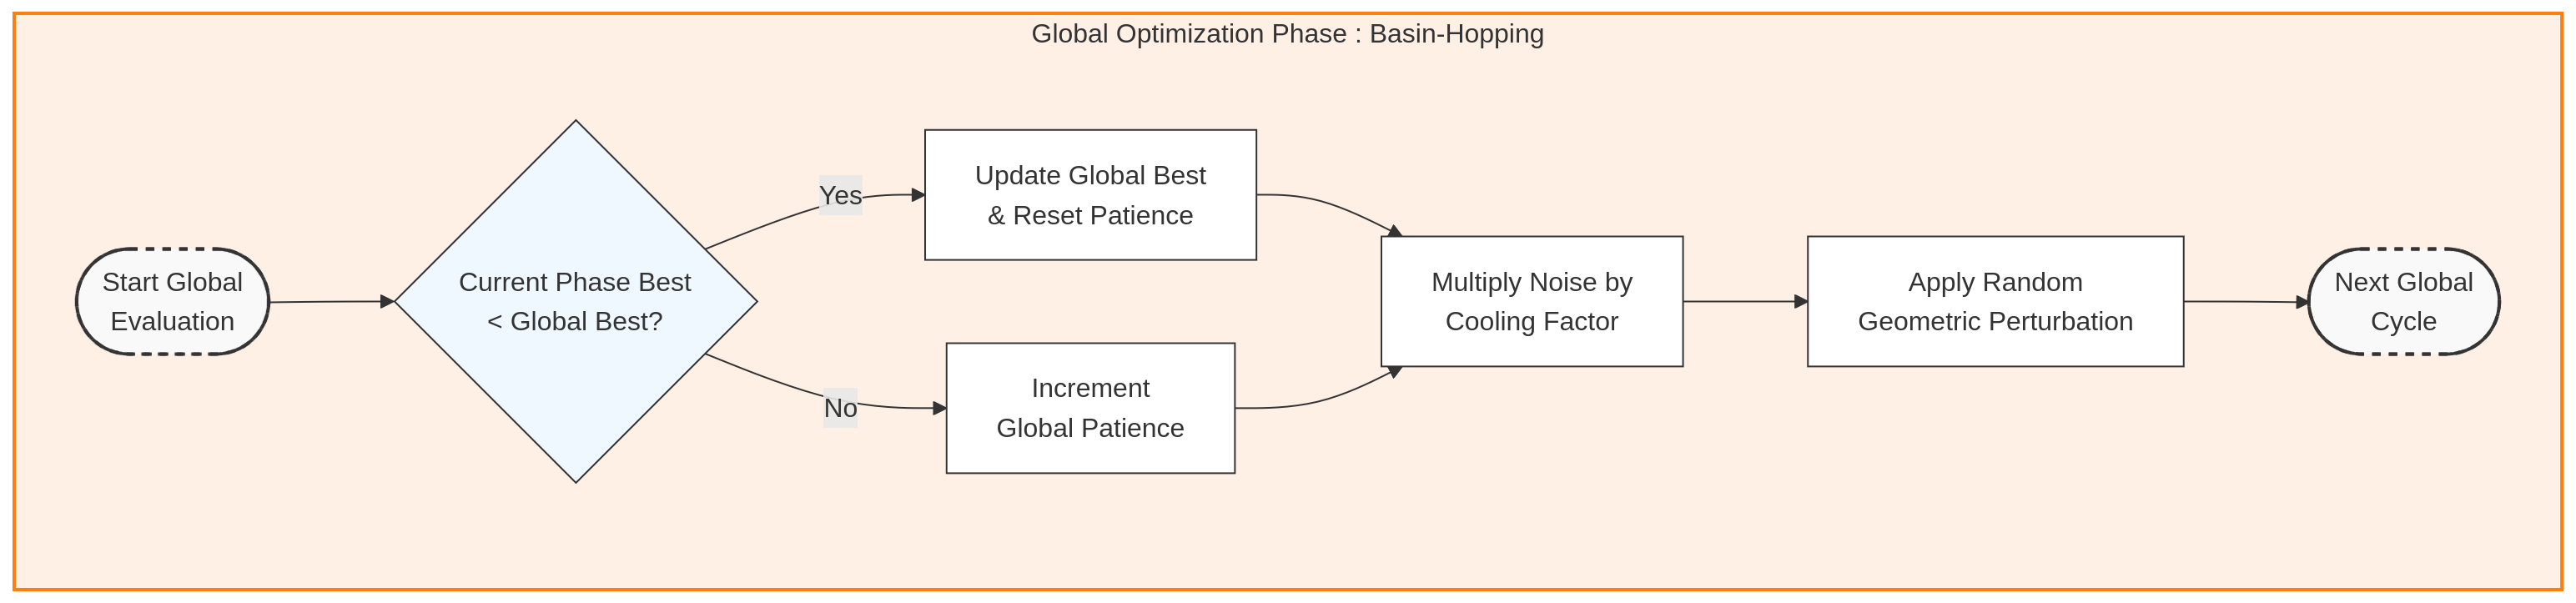
\includegraphics[width=0.9\linewidth]{diagrams/global_optim.png}
    \caption{Global optimization phase (basin-hopping perturbation).}
    \label{fig:global-optim}
\end{figure}

\subsection{Complete Pipeline}

In addition of the optimization algoritm, there are some steps before and after it to prepare the inputs and the outputs of the optimization (see Fig. \ref{fig:complete-pipeline}). Before the optimization phase, the coarse-gained model must be instantiated with starting spatial coordinates for its virtual beads. The molecule is generated as a simple linear chain, with adjacent beads separated by an equilibrium bond distance. This equilibrium bond distance was obtained from statistical analyse. We retrieved all RNA with a resolution inferior at 1.0 \r{A}  from the PDB and we extract every inter-distance from one atom particulary (eg : C3' or C4')  and we used the mean.  With this phase, the strucutre is a linear, considering neutral, and can be used at a starting point for the optimization phase. 

After the optimization phase, we obtain a PDB file with only the coordinate of the reference atom. To passing to a coarse-gained representation to a full-atom representation, we passed the strucuture into a software ARENA \cite{perry_arena_2023}. The software will maps ideal nucleobase and sugar-phosphate templates onto the optimized strucure obtained. 

Finally after the full-atom reconstruction, we used to tools AMBER14 \cite{amber14} force fiel within the OpenMM \cite{openmm} simulation framework to ensure strict thermodynamic realism and to resolve any residual steric clashes. 

At the end of this pipeline, the result is a highly refined, all-atom structural model and exported into standard structural biology formats.

\begin{figure}[h!]
    \centering
    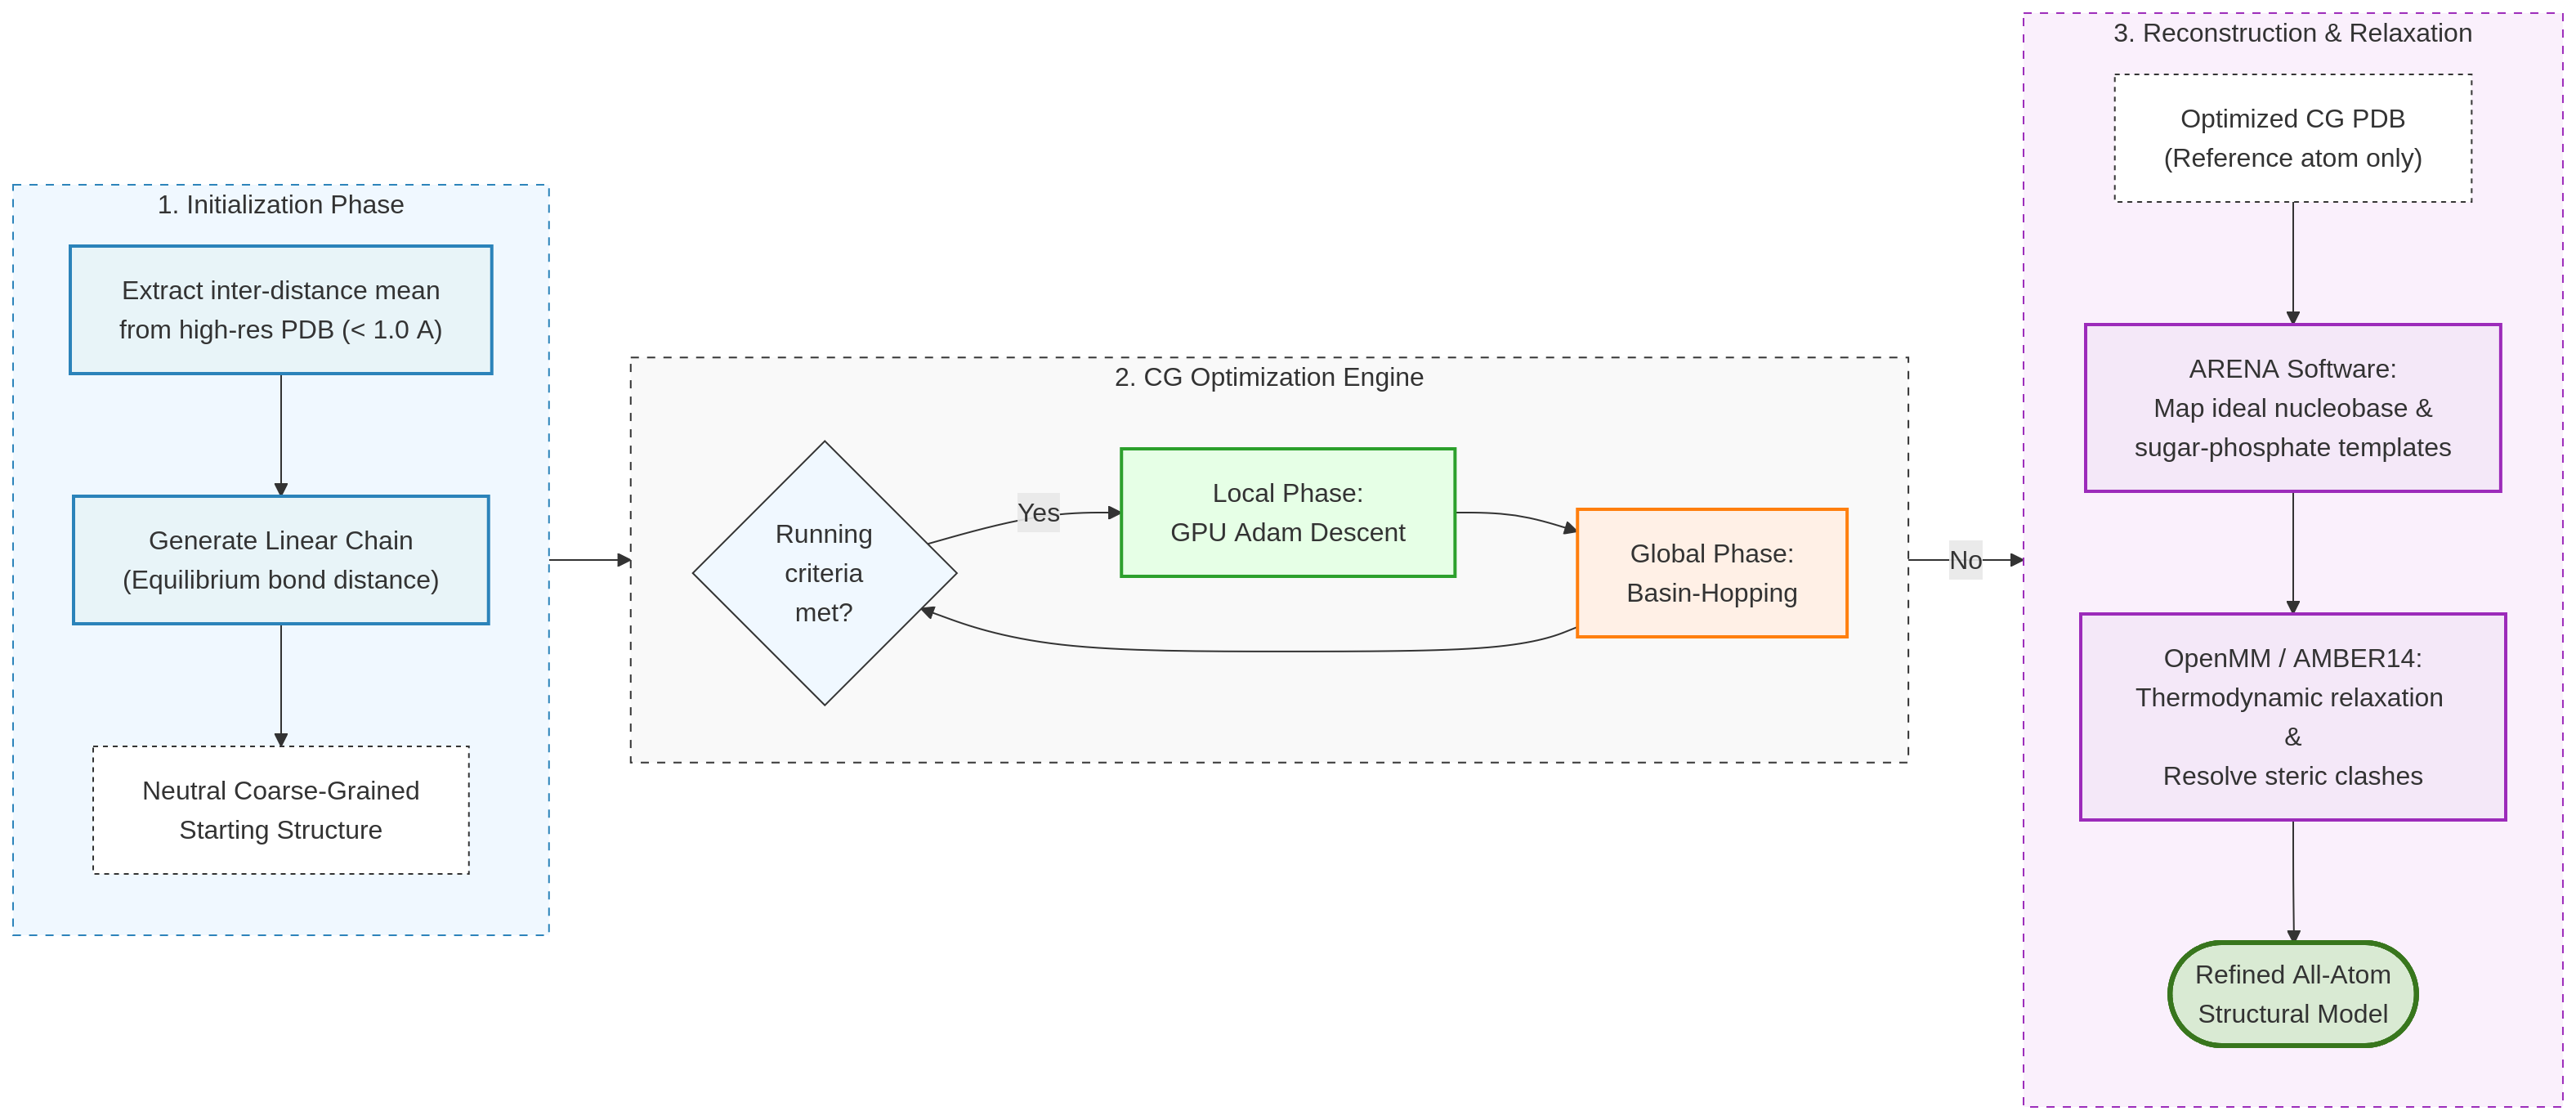
\includegraphics[width=\linewidth]{diagrams/complete_pipeline.png}
    \caption{Complete Pipeline of the all prediction algorithm.}
    \label{fig:complete-pipeline}
\end{figure}


\subsection{Different Applications}

Beyond the prediction of RNA three-dimensional structures, the proposed algorithmic framework can be repurposed for dynamic structural analysis. Because the core optimization engine, driven by the Adam gradient descent, relies on a continuously differentiable objective function, the knowledge-based statistical potential can be substituted with a purely geometric metric, such as the \acrfull{rmsd} relative to a known experimental target. By minimizing this derivable distance metric instead of thermodynamic energy, the optimization algorithm will calculate gradients that guide the spatial coordinates toward the target state. Recording this stepwise convergence generates a continuous structural trajectory, effectively producing a computational \textit{movie} of the simulated folding pathway.

Furthermore, this methodology can be extended to investigate complex RNA conformational dynamics. Instead of initializing the optimization algorithm from a linear chain, the coarse-grained model can be seeded with the coordinates of a natively folded state, while setting a different known conformation of the exact same RNA as the RMSD target. So the optimization algorithm will produce the structural transition between the two topologies. Consequently, the framework can be utilized to simulate and observe conformational switches

% ==========================================
% Results
% ==========================================
\section{Results}
\subsection{Interpolation results}
\subsection{Comparaison between original and predicted structures}
\subsection{Comparatives tables}
\subsection{Line chart of score function for folding trajectory}
\subsection{Internet platform for RNA folding}
% ==========================================
% Discussion
% ==========================================
\newpage
\section{Discussion and Perspectives}


% ==========================================
% Conclusion
% ==========================================
\newpage
\section{Conclusion}


% ==========================================
% Annexe/Glossary
% ==========================================

\newpage

\label{glossaire}
%  vocabulaire technique, avec définition et page où est utilisé le mot la première fois
\thispagestyle{plain}
\setglossarystyle{listhypergroup}
% \setglossarystyle{index} % not combine by group
\glsaddallunused % change line
\printnoidxglossaries

% ==========================================
% References
% ==========================================
\newpage
\addcontentsline{toc}{section}{References}
\printbibliography[type=article,title={Articles}]

\addcontentsline{toc}{section}{Websites}
\printbibliography[nottype=article,title={Websites}]

% ==========================================
% List figures Tables
% ==========================================
\newpage

\thispagestyle{empty}
\addcontentsline{toc}{section}{List of figures}
\listoffigures
\addcontentsline{toc}{section}{List of tables}
\listoftables

\end{document}
